\documentclass[
  a4paper,            % DIN A4
  DIV=10,             % Schriftgröße und Satzspiegel
  oneside,            % einseitiger Druck
  BCOR=5mm,           % Bindungskorrektur
  parskip=half,       % Halber Abstand zwischen Absätzen
  numbers=noenddot,   % Kein Punkt hinter Kapitelnummern
  bibtotoc,           % Literaturverzeichnis im Inhaltsverzeichnis
  listof=totoc        % Abbildungs- und Tabellenverzeichnis im Inhaltsverzeichnis
]{scrartcl}
\usepackage{../style/termpaperstyle}

%\usepackage{layout}       % Layout Debugging
%\usepackage{showframe}    % Layout Debugging
\usepackage{lipsum}       % for example only
\usepackage{blindtext}    % for example only
\usepackage{listings}
\usepackage{color}

\usepackage{placeins}

\definecolor{mygreen}{rgb}{0,0.6,0}
\definecolor{mygray}{rgb}{0.5,0.5,0.5}
\definecolor{mymauve}{rgb}{0.58,0,0.82}

\lstset{ 
  backgroundcolor=\color{white},   % choose the background color; you must add \usepackage{color} or \usepackage{xcolor}; should come as last argument
  basicstyle=\footnotesize,        % the size of the fonts that are used for the code
  breakatwhitespace=true,         % sets if automatic breaks should only happen at whitespace
  breaklines=true,                 % sets automatic line breaking
  captionpos=b,                    % sets the caption-position to bottom
  commentstyle=\color{mygreen},    % comment style
  deletekeywords={...},            % if you want to delete keywords from the given language
  escapeinside={\%*}{*)},          % if you want to add LaTeX within your code
  extendedchars=true,              % lets you use non-ASCII characters; for 8-bits encodings only, does not work with UTF-8
  firstnumber=0,                % start line enumeration with line 1000
  frame=single,	                   % adds a frame around the code
  keepspaces=true,                 % keeps spaces in text, useful for keeping indentation of code (possibly needs columns=flexible)
  keywordstyle=\color{blue},       % keyword style
  language=python,                 % the language of the code
  morekeywords={*,...},            % if you want to add more keywords to the set
  numbers=left,                    % where to put the line-numbers; possible values are (none, left, right)
  numbersep=5pt,                   % how far the line-numbers are from the code
  numberstyle=\tiny\color{mygray}, % the style that is used for the line-numbers
  rulecolor=\color{black},         % if not set, the frame-color may be changed on line-breaks within not-black text (e.g. comments (green here))
  showspaces=false,                % show spaces everywhere adding particular underscores; it overrides 'showstringspaces'
  showstringspaces=false,          % underline spaces within strings only
  showtabs=true,                  % show tabs within strings adding particular underscores
  stepnumber=2,                    % the step between two line-numbers. If it's 1, each line will be numbered
  stringstyle=\color{mymauve},     % string literal style
  tabsize=4,	                   % sets default tabsize to 4 spaces
  title=\lstname                   % show the filename of files included with \lstinputlisting; also try caption instead of title
}
\usepackage{booktabs}
\begin{document}
% !TEX root = ../termpaper.tex
%
% configurations
%

% text field
%-> replace supervisor names with correct ones
\firstSupervisor{Prof. Dr.-Ing. Hans-Dieter Schütte}
\secondSupervisor{}    % only if needed, otherwise left blank

% text field
%-> replace title with your title of the seminar work
\termPaperTitle{Entwurf und Simulation einer hochselektiven Filterbank in Brückenstruktur mit Python}
\termPaperTitleEN{Design and simulation of a highly selective filter bank in bridge structure with Python}

% text field
%-> replace the key words with your own key words or remove the words
\keywordsDE{Digitale Signalverarbeitung, Wellendigitalfilter, Oktav-Filterbank, Simulation}
\keywordsEN{Digital signal processing, Wave digital filter, Octave filterbank, Simulation}

% text field
%-> replace jon with your name
\termPaperAuthor{Erik Engelhardt, Christopher Rotzlawski}

% text field
%-> enter the submission date
\submissionDate{18. Juni 2019}

% switch - uncomment only one
%-> uncomment NDA or public
%\NDA{yes}
\NDA{no}

%-> uncomment cover or cover Corporate Design 2017
%\Cover{CD2017}
%\Cover{CD2017NoLogo}
\Cover{Std2018}

% switch - uncomment only one
%-> uncomment the kind of seminar you are in
\seminarKind{S}     % seminar in bachelor course
%\seminarKind{Pro}   % pro-seminar in bachelor course
%\seminarKind{GSem}  % foundation seminar in master computer science
%\seminarKind{HSem}  % main seminar in master computer science

% switch - uncomment only one
%-> uncomment the study course you are in
\studycourse{TI}
%\studycourse{AI}
%\studycourse{WI}
%\studycourse{EI}
%\studycourse{BMT}
%\studycourse{MAI}  % master in computer science
%\studycourse{MIK}
%\studycourse{MA}  

    % load all settings

%\layout{}                 % Layout Debugging

\hyphenation{Ba-che-lor-the-sis Mas-ter-the-sis}

% Cover page here, no page number
\ICoverPage

% Titlepage is page one even if the number is not shown.
\pagenumbering{roman}

% Table of contents here
\newpage
\tableofcontents

% Uncomment if list of source code is needed (rarely).
%\lstlistoflistings  % requires package listings, needs to uncommenting of usepackage

% path to the chapters folder is set to find the images used there
\graphicspath{ {./chapters/} }

% Chapters
\clearpage
\pagenumbering{arabic}

%\begin{abstract}
%% !TEX root = ../termpaper.tex
% first example for the abstact
% @author Thomas Lehmann
%
\vspace*{0.4cm}

\noindent Der vorliegende Text ist ein Beispiel für eine Seminararbeit und soll nur die Verwendung des Templates aufzeigen.

%\end{abstract}

\ITextBlockKeywords

% !TEX root = ../termpaper.tex
% first example sections
% @author Thomas Lehmann
%

\section{Einleitung}


% !TEX root = ../termpaper.tex
% first example sections
% @author Thomas Lehmann
%

\section{Grundlagen}
Im folgenden Kapitel wird auf die Grundlagen eingegangen, die in Zusammenhang mit diesem Projekt stehen. Dabei handelt es sich um den bireziproken Teilbandfilter und der Oktav-Filterbank.

\subsection{Bireziproker Teilbandfilter}
Die Grundstruktur des bireziproken Filters sind Wellendigitalfilter. Wellendigitalfilter sind dabei Filter der digitalen Signalverarbeitung, die auch unter nicht linearen Bedingungen eine gute Stabilitätseigenschaft aufweisen \cite[vgl.][S. 68]{gaszi1983}.\par
Bei den bireziproken Filtern, auch selbstreziproke Filter genannt, handelt es sich um eine Unterklasse der Wellendigitalfilter. Bei dem Filterdesign dieser Filter kann entweder die Durchlassdämpfung oder die Sperrdämpfung frei gewählt werden, da der Frequenzbereich bis $\frac{F_s}{4}$ nicht unabhängig von dem Bereich von $\frac{F_s}{4}$ bis $\frac{F_s}{2}$ ist \cite[vgl.][S. 72]{gaszi1983}.\par
Die Anzahl der Adaptoren innerhalb des Filters ist dabei geringer als bei üblichen Wellendigitalfiltern. Bireziproke Filter umfassen $\frac{N - 1}{2}$ Adapter \cite[vgl.][S. 73]{gaszi1983}.\par
Für dieses Projekt wird der bireziproke Filter aus \cite{gaszi1983} verwendet. Hierbei handelt es sich um einen Filter 19. Grades mit Cauer-Parametern. Das Filterdesign und die Berechnung der Cauer-Parameter ist in \cite[][S. 74]{gaszi1983} zu finden.\par
Die Grundstruktur des Filters setzt sich wie in Abbildung \ref{fig:bireziprok_Struktur} aus neun Adaptoren zusammen. Da es bei der Simulation zu keinem Überlauf der Variablen kommen kann und in diesem Zusammenhang die Größe der berechneten Cauer-Parameter keine Auswirkung hierauf haben, wird die Filterstruktur vereinfacht, indem neun gleiche Adaptore verwendet werden. Hierfür wird der Adaptor für einen $\gamma$-Bereich von $0\leq\gamma\leq0,5$ verwendet, da hier die Beziehung von $\alpha=\gamma$ gilt (siehe Abbildung \ref{fig:Adaptor}).
\begin{figure}[h!]
	\centering	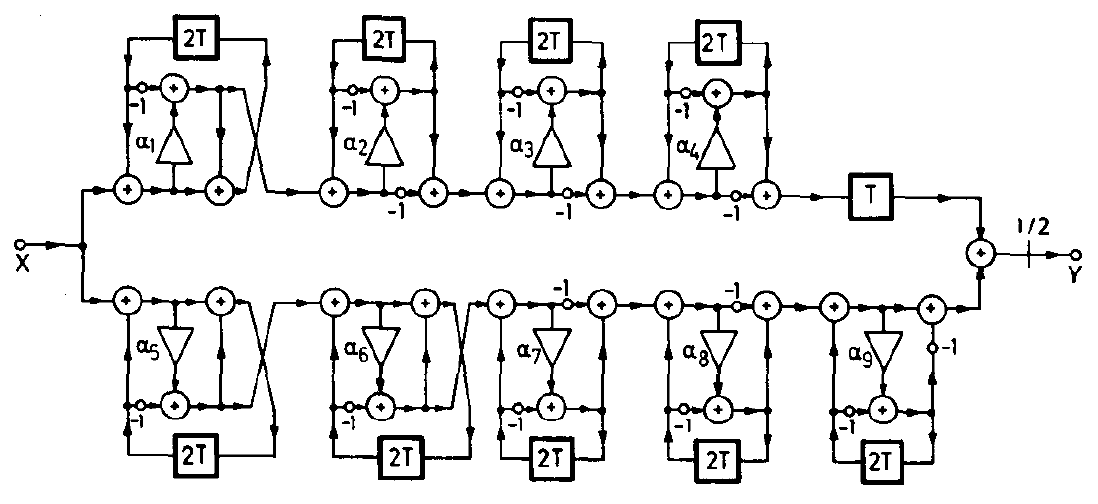
\includegraphics[width=15cm]{img/BireziprokerFilter.png}
	\caption{Grundstruktur des bireziproken Wellendigitalfilters \cite[][S. 85]{gaszi1983}}
	\label{fig:bireziprok_Struktur}
\end{figure}
\begin{figure}[h!]
	\centering	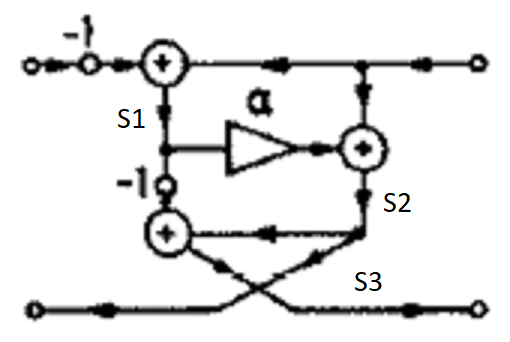
\includegraphics[width=10cm]{img/Adapter.png}
	\caption{Verwendeter Adaptor für den bireziproken Wellendigitalfilter \cite[][S. 77]{gaszi1983}}
	\label{fig:Adaptor}
\end{figure}

\subsection{Oktav-Filterbank}
Bei der Oktav-Filterbank handelt es sich um einen Filter, welcher aus mehreren Brücken-Wellendigitalfiltern besteht. Herbei besitzt jedes Teilbandfilter einen Tief- und Hochpassausgang. Somit ergibt sich, dass je Teilbandfilter das Frequenzband halbiert wird \cite[vgl.][S. 90]{kunold1989}.\par
Um bei jeder Teilbandfilterstufe das Signal jeweils in einen höherfrequenten und niederfrequenten Teil zu trennen, ist eine Filtertransformation nötig. Dies geschieht mit den folgenden Beziehungen:
\begin{equation}
\psi = \frac{z - 1}{z + 1}
\end{equation}
\begin{equation}
\psi' = \frac{2 \psi}{1 + \psi^2} = \frac{2 \left(\frac{z - 1}{z + 1}\right)}{1 + \left(\frac{z - 1}{z + 1}\right)^2} = \frac{z^2 - 1}{z^2 - 1}
\end{equation}
\begin{equation}
z' = z^2
\end{equation}
\begin{equation}
z^{'-1} = z^{-2}
\end{equation}
Somit folgt, dass mit jeder Teilbandfilterstufe die jeweiligen Delays des Filters verdoppelt werden.\par
Da bei jedem Teilfilterdurchlauf ein zusätzlich Delay erzeugt wird, besitzen die neun Teilbänder unterschiedliche Signallaufzeiten. Dies muss durch zusätzliche Delayglieder in den Teilbändern kompensiert werden, damit am Aus- und Eingang der Oktav-Filterbank ein identisches Signal anliegt.\par
Für dieses Projekt wird eine Oktav-Filterbank mit neun Teilbändern nach \cite[][]{kunold1989} verwendet (siehe Abbildung \ref{fig:OktavFilterbank}). Des Weiteren werden die linearphasigen Teilbandfilter gegen bireziproke Teilbandfilter ausgetauscht.
\begin{figure}[h!]
	\centering	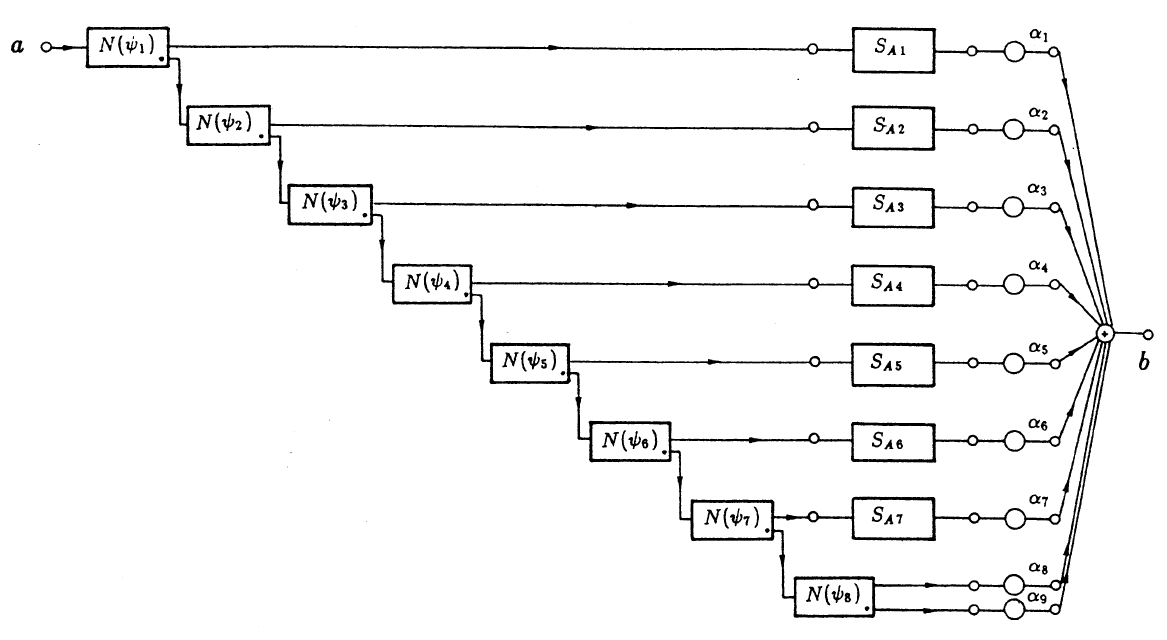
\includegraphics[width=15cm]{img/OktavFilter.png}
	\caption{Oktav-Filterbank mit neun Teilbändern \cite[][S. 95]{kunold1989}}
	\label{fig:OktavFilterbank}
\end{figure}
%%% Local Variables:
%%% mode: latex
%%% TeX-master: "../termpaper"
%%% End:

\section{Implementierung}
In diesem Kapitel wird die Implementierung der hochselektiven Filterbank in Python 3.7 beschrieben.

\subsection{Übersicht}\label{sec:impl_ueber}

\subsubsection{Verwendete Bibliotheken}\label{sec:impl_bib}
Für einige Berechnungen und das Speichern von Datenstruckturen wurde das Numpy Modul der Scipy Bibliothek~\cite{scipy} verwendet. Für das Erstellen der Diagramme wurde die Matplotlib Bibliothek~\cite{Hunter:2007}.
\subsubsection{Klassendiagramm}\label{sec:impl_klass}
\begin{figure}
  \centering
  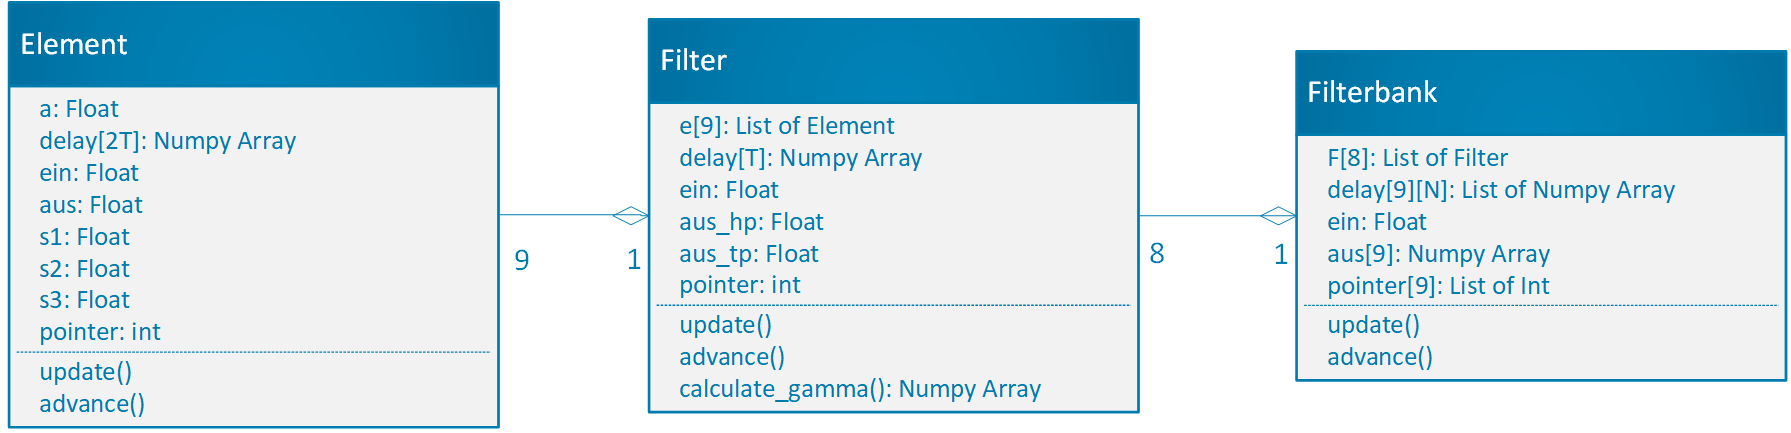
\includegraphics[width=1\textwidth]{img/klassendia}
  \caption{Klassendiagramm für die Implementierung einer hochselektiven Filterbank}\label{fig:impl_klassdia}
\end{figure}
Wie in Abbildung~\ref{fig:impl_klassdia} zu sehen erfolgt die Implementierung der hochselektiven Filterbank objektorientiert. Dabei besteht eine Filterbank aus 8 Filtern (vgl. Abb. TODO) und ein Filter aus 9 Elementen (vgl. Abb.).
\subsection{Klassen}\label{sec:impl_klassen}
Im folgenden wird die Implementierung der Klassen im einzelnen beschrieben bevor im nächsten Unterkaptitel auf dei verwendeten Testfunktionen eingegangen wird.
\subsubsection{Element}\label{sec:impl_ele}
Ein Element (s. Lst.~\ref{lst:element}) stellt den kleinsten Teil der Filterbank dar. Neben Ein- und Ausgang verfügt ein Element über ein Delay-Array dessen Länge bei der Initialisierung übergeben werden kann. Hierüber lässt sich die Ordnung des Teilfilters einstellen (vlg. Kap. TODO). Außerdem muss bei der Initialisierung ein Wert für \emph{a} übergeben werden. Dieser bestimmt mit welchem Wert im Element multipliziert wird (vlg. Abb. TODO).

Über das Aufrufen der Funktion \emph{update()} werden die Summen und der Ausgang des Elements neu berechnet. Die Funktion \emph{advance()} wird verwendet um einen Takt des Systems zu simulieren. Der Pointer, welcher den aktuellen Eingang des Verzögerungsgliedes anzeigt wird inkrementiert und ein neuer Wert wird in das Array geschrieben. Der aktuell gültige Augang des Verzögerungsarrays befindet sich eine Stelle \emph{vor} dem Eingang (vgl. Lst.~\ref{lst:element} Zeile 16).

\lstinputlisting[language=Python, firstline=6, lastline=31, caption={Quellcode der Klasse Element}, label={lst:element}]{list/wellendigitalfilter.py}


\subsubsection{Filter}\label{sec:impl_Filter}
Ein Teilfilter (s. Lst.~\ref{lst:filter}) besteht aus 9 Elementen und einem Verzögerungsglied (vlg. Abb. TODO). Bei der Initialisierung muss kann die Anzahl der Verzögerungen und damit die Ordnung des Teilfilters übergeben werden. Die Koeffizienten der Elemnte gemäß~\cite{gaszi1983} über die Funktion \emph{calculate\_gamma(fs, F)} berechnet. Wobei \emph{F} die Taktfrequenz des Systems und \emph{fs} die gewünschte Stopfrequenz des Filters ist.

Ü
\lstinputlisting[language=Python, firstline=34, lastline=118, caption={Quellcode der Klasse Filter}, label={lst:filter}]{list/wellendigitalfilter.py}

\subsubsection{Filterbank}\label{sec:impl_bank}
\lstinputlisting[language=Python, firstline=121, lastline=160, caption={Quellcode der Klasse Filterbank}, label={lst:bank}]{list/wellendigitalfilter.py}
\subsection{Testfunktionen}\label{sec:impl_test}

\subsubsection{Test Filter}\label{sec:impl_testFilter}
\lstinputlisting[language=Python, firstline=163, lastline=193, caption={Quellcode der Testfunktion für einen einzlnen Filter}, label={lst:test_filter}]{list/wellendigitalfilter.py}
\subsubsection{Test Filterbank}\label{sec:impl_testBank}
\lstinputlisting[language=Python, firstline=196, lastline=236, caption={Quellcode der Testfunktion für die gesamte Filterbank}, label={lst:test_bank}]{list/wellendigitalfilter.py}
%%% Local Variables:
%%% mode: latex
%%% TeX-master: "../termpaper"
%%% End:

% !TEX root = ../termpaper.tex
% first example sections
% @author Thomas Lehmann
%

\section{Simulation}
Im folgenden Kapitel werden die Simulationsergebnisse der hochselektiven Filterbank analysiert.

\subsection{Simulation der Teilbandausgänge}
Zunächst werden die Ausgänge der einzelnen Teilbänder simuliert. Hierzu werden die neun Ausgänge einzeln über den Frequenzbereich geplottet.\par
Abbildung \ref{fig:Teilband0} zeigt den Ausgang des ersten Teilbandes. Hier ist zu sehen, dass der Durchlassbereich bei den Frequenzen von $\frac{F_s}{4}$ bis $\frac{F_s}{2}$ liegt und somit gewünschte Hochpassverhalten zeigt.\par
\begin{figure}[h!]
	\centering	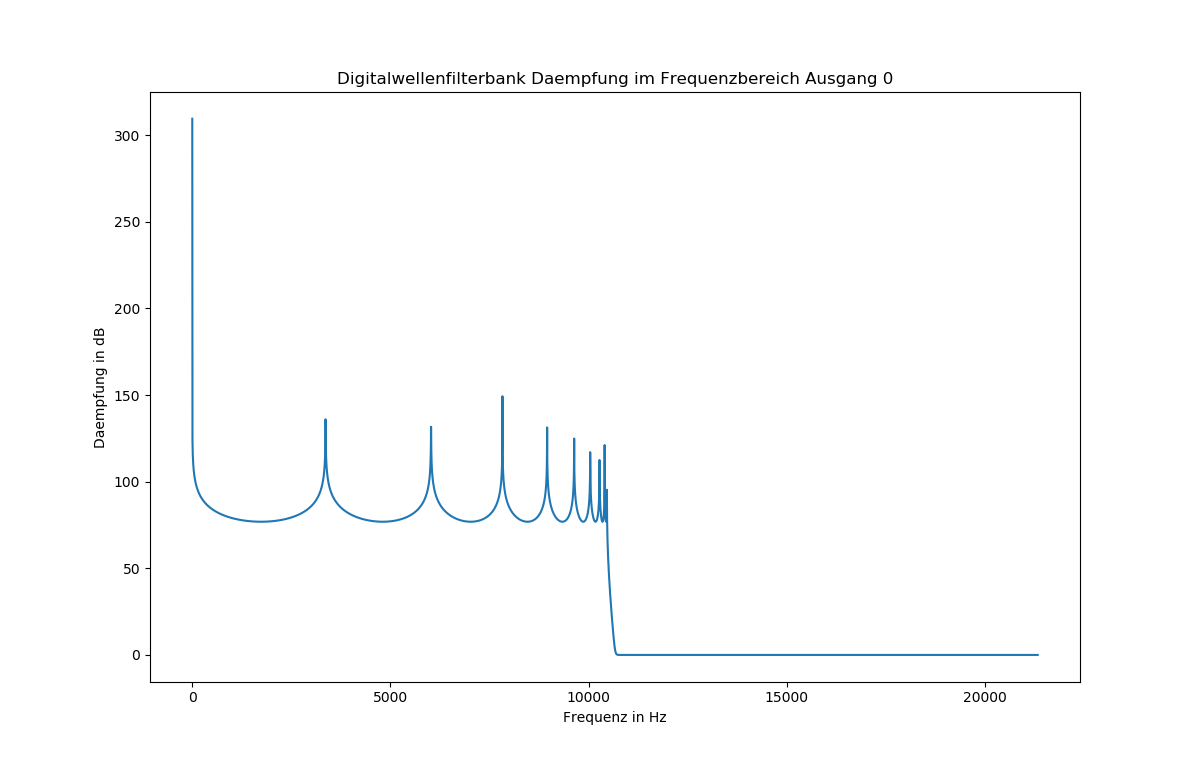
\includegraphics[width=14cm]{img/bank_freq_0.png}
	\caption{Ausgang des ersten Teilbandes}
	\label{fig:Teilband0}
\end{figure}
Ein weiteres exemplarisches Teilband zeigt Abbildung \ref{fig:Teilband5} mit dem sechsten Teilband. Hierbei ist der erkennen, dass das Teilband den erwarteten Frequenzbereich von 375 bis 750\,Hz durchlässt.\par
\begin{figure}[h!]
	\centering	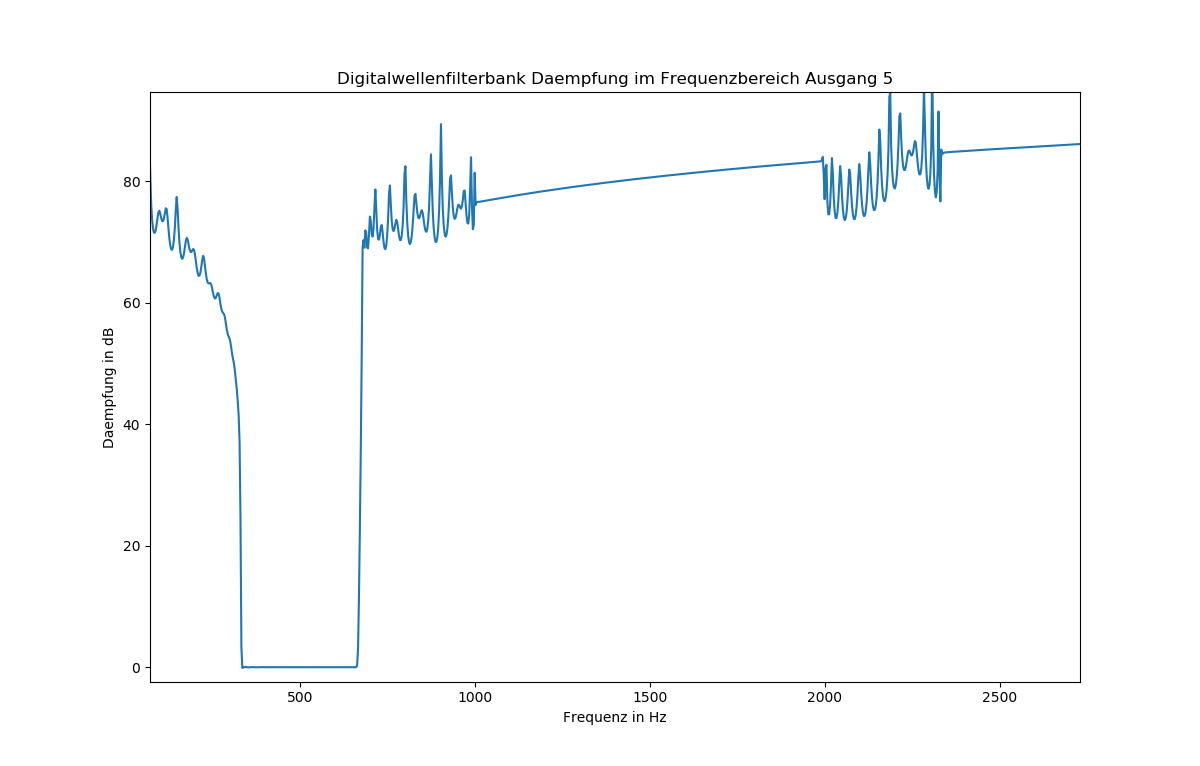
\includegraphics[width=14cm]{img/bank_freq_5_close.png}
	\caption{Ausgang des sechsten Teilbandes}
	\label{fig:Teilband5}
\end{figure}
Die restlichen Teilbänder zeigen ebenfalls den erwarteten Durchlassbereich.

\subsection{Simulation der Signallaufzeiten}
Nachfolgend werden die Signallaufzeiten der einzelnen Teilbänder simuliert und in einem zusammen in einem Plot dargestellt (siehe Abbildung \ref{fig:TeilbandLaufzeitenohne}). Zu erkennen ist, dass ein Ausgleich der einzelnen Signallaufzeiten nötig ist.\par
\begin{figure}[h!]
	\centering	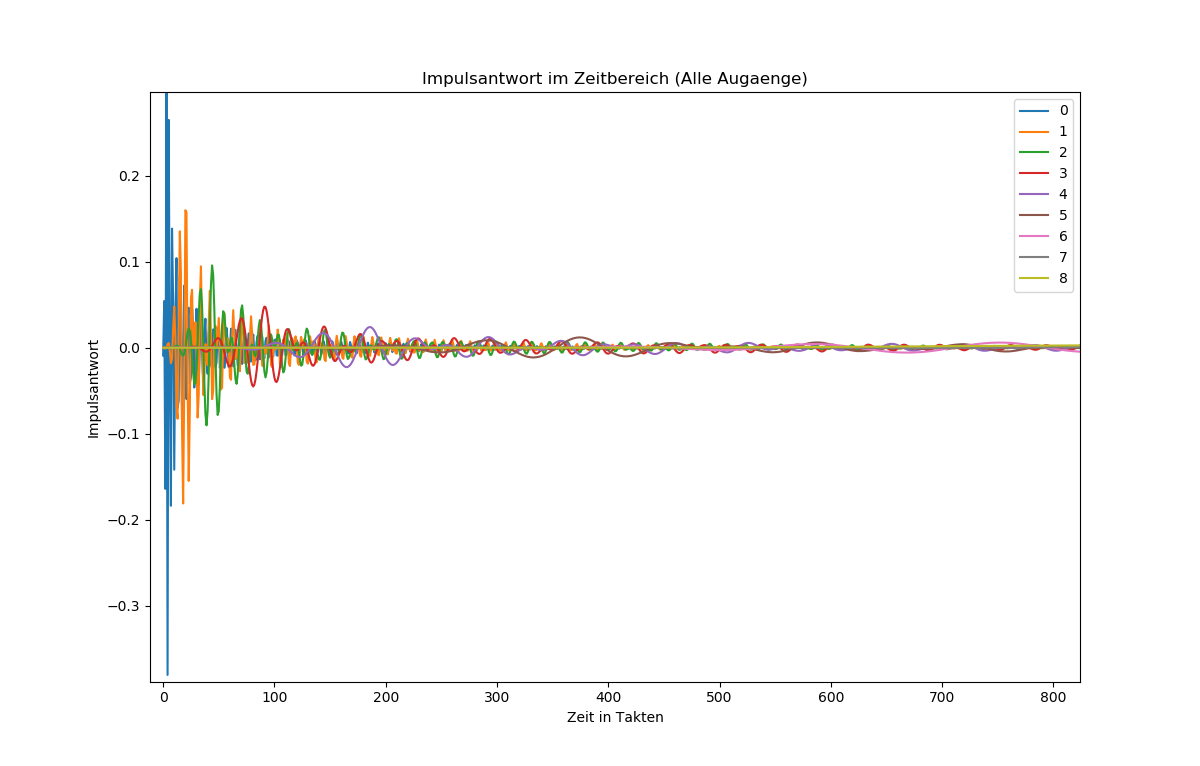
\includegraphics[width=15cm]{img/bank_zeit_alle_keinAusgleich.png}
	\caption{Signallaufzeiten der Teilfilterbänder ohne Ausgleich}
	\label{fig:TeilbandLaufzeitenohne}
\end{figure}
Die einzelnen laufzeitbereinigten Impulsantworten der Teilbänder zeigen das Maximum ungefähr nach 1500 Takten (siehe Abbildung \ref{fig:TeilbandLaufzeiten}). Somit kann das ursprüngliche Signal am Ausgang wieder zusammengesetzt werden.
\begin{figure}[h!]
	\centering	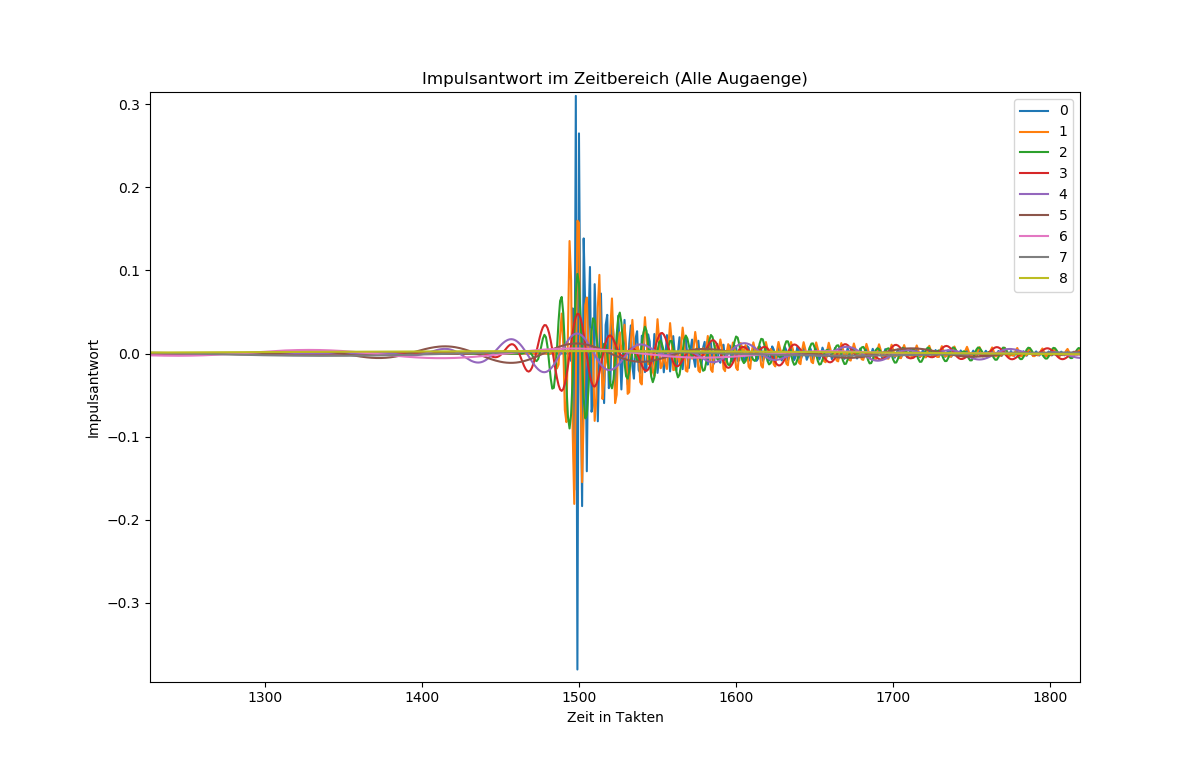
\includegraphics[width=15cm]{img/bank_zeit_alle.png}
	\caption{Signallaufzeiten der Teilfilterbänder}
	\label{fig:TeilbandLaufzeiten}
\end{figure}

\subsection{Simulation des Oktav-Filterbank-Ausgangs}

\begin{figure}[h!]
	\centering	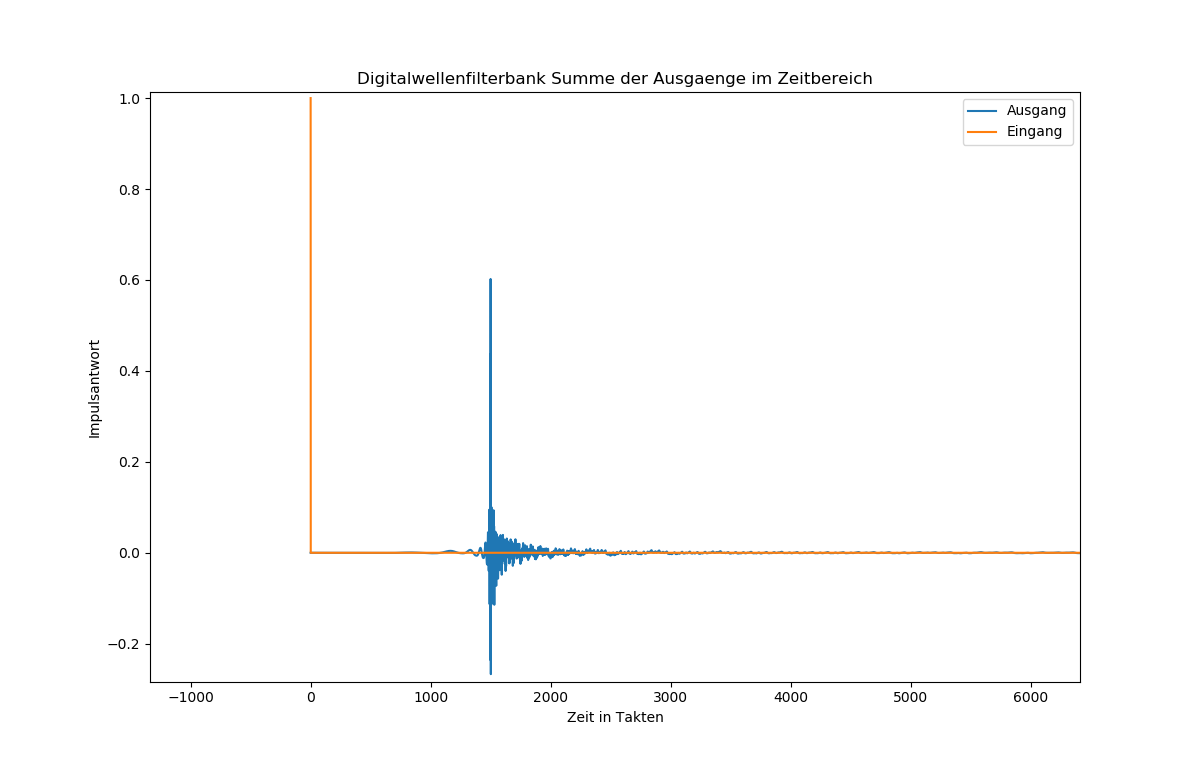
\includegraphics[width=14cm]{img/bank_zeit_summe.png}
	\caption{Signallaufzeit der Summe der Teilbänder}
	\label{fig:OktavLaufzeit}
\end{figure}

\begin{figure}[h!]
	\centering	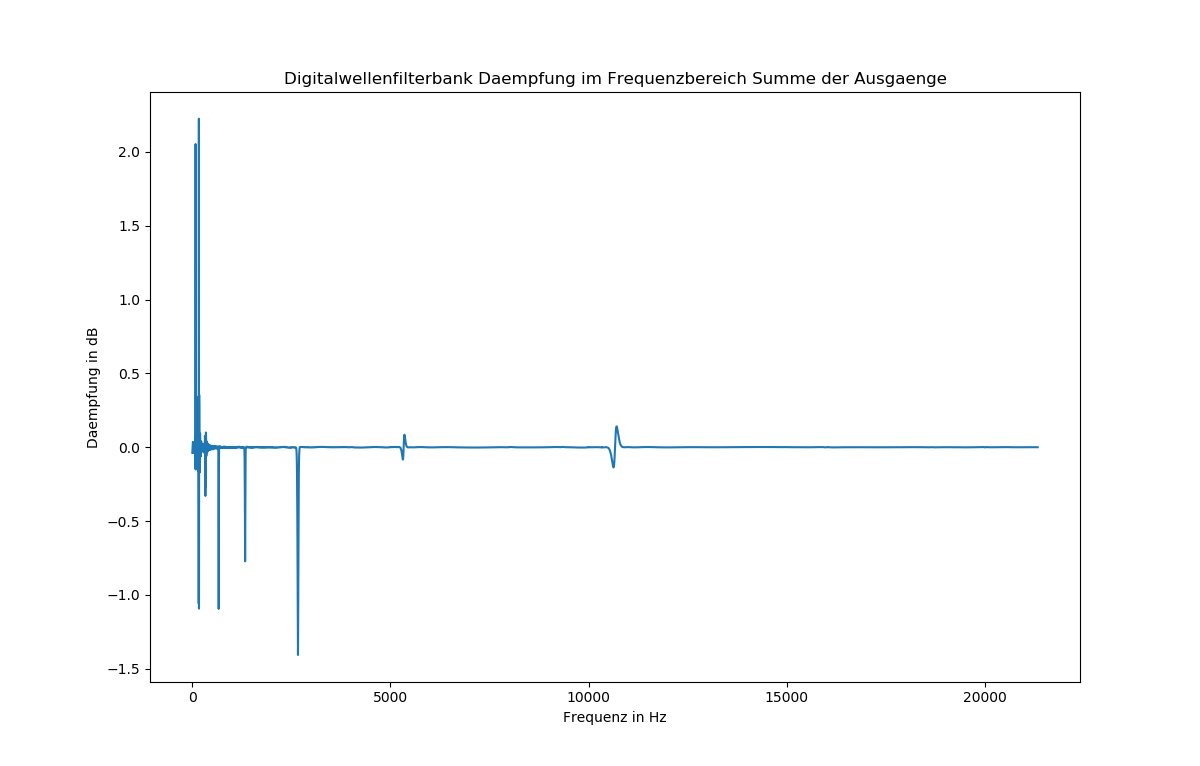
\includegraphics[width=14cm]{img/bank_freq_summe.png}
	\caption{Dämpfung der Oktav-Filterbank}
	\label{fig:AusgangDeampfung}
\end{figure}
% !TEX root = ../termpaper.tex
% first example sections
% @author Thomas Lehmann
%

\section{Fazit}

% Add additional chapters here

%\bibliographystyle{plain}
\bibliographystyle{dinat}
\bibliography{literature}

%\Istatement

\end{document}

%%% Local Variables:
%%% mode: latex
%%% TeX-master: t
%%% End:
